\newpage
\section{Prinsipiell løsning}
\label{prinsipiellLoesning}

Ettersom det er ønskelig med så høy ingagnsmotstand og så lav utgagngsmotstand som mulig så er et Darlington par et godt valg. Et Darlington par er to NPN-transistorer koblet sammen som vist i figur \ref{fig:Darlington_basic}. Darlington par kan ses på som en enkelt transistor med en strømforsterkning lik produktet av de to transistorene.

\begin{figure}[H]
\centering
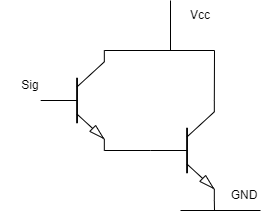
\includegraphics[scale=0.5]{bilder/Darlington_basic.drawio.png}
\caption{Darlington par}
\label{fig:Darlington_basic}
\end{figure}

Darlington paret har en strømforsterkning på $\beta_1 \cdot \beta_2$ og en inngangsmotstand på $\beta_1 \cdot R_{B1}$. Utgangsmotstanden er lik $R_{C2}$.

For å kunne lage en enkel buffer ut av et Darlington par så må det legges til en emittermotstand, inn- og utgangs kondensatorer i tilleg til at arbeidspunktet burde settes til midten av spenningsforsyningen. Dette er vist i figur \ref{fig:Darlington_buffer}. Forsterkningen måles mellom inngagnssignalet $V$ og utgangssignalet $V_2$.

\begin{figure}[H]
\centering
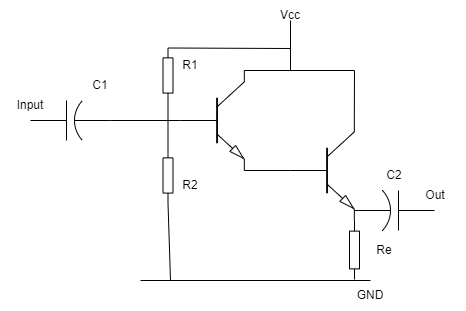
\includegraphics[scale=0.8]{bilder/Darlington_buffer.drawio.png}
\caption{Darlington buffer}
\label{fig:Darlington_buffer}
\end{figure}



